\comseb{Sur le plan (pas évident de mettre un commentaire sur le plan: marrant que tu sautes des probas aux probas imprécises pour revenir aux possibilités. J'aurais peut-être fait une section générique (probas, ensembles, ensembles aléatoires, ensembles de probas?), puis un focus sur possibilités? J'aurais sans doute aussi séparé ce qui est modélisation (3.2/3.3 dans le 2) de ce qui est plus calculatoire (2.5 dans 3)? Commencer par une intro, finir par une conclusion/perspective}

\chapter{Introduction to stereophotogrammetry}



\comroman{TODO: Prendre le lecteur par la main, lui expliquer ce qu'il va lire et pourquoi dans cet ordre là \etc. Biblio sur la photogrammetry, l'utilité des DSM, la description des pipelines de photogrammetry, uncertainty dans les DSM.}

\section{Digital Surface Models}
Knowing the Earth's topography is crucial for modern geosciences. As such, \acrfull{dsm}, which are a representation of a surface's elevation on a regular grid, appear as a natural solution in many \acrfull{gis}. Indeed, they can easily be handled and provide georeferenced information regarding the topography of an area. \acrshort{dsm} find usage in various contexts for a wide range of applications. In \acrfull{eo} for instance, \acrshort{dsm} are used to monitor changes in vegetation \cite{sadeghi_canopy_2016}, melting rates of glaciers \cite{berthier_glacier_2014, rieg_pleiades_2018}, volcanos \cite{ganci_data_2022}, snow or water resources \cite{marti_mapping_2016, yamazaki_merit_2019} \etc Similarly, \acrshort{dsm} are employed for catastrophe management, to predict the potential damage caused by earthquakes or floods \cite{jenkins_physics-based_2023} \dots \acrshort{dsm} are also crucial for ortho-rectifying images, \ie transforming images so that their scale becomes uniform. It allows images to be easily used in GIS or as background for maps. In urban settings, high resolution \acrshort{dsm} can be help drone navigation for Defense applications, or more broadly for urban planning \cite{velazco_3d_2012}.

Nowadays, \acrshort{dsm} are mostly generated from laser scanning with LiDAR sensors, radar interferometry or stereophotogrammetry \cite{youssefi_cars_2020}. Air-borne laser scanning results in \acrfull{vhr} models, but the swath width and cost of acquisition campaigns do not allow to periodically cover the globe. Space-borne \acrshort{lidar} is mostly used for atmospheric measurements, or discrete measurements \cite{fouladinejad_history_2019} \comroman{Et parler de ICESAT-2}. Space-borne radar interferometry remains widely used, and has allowed to create a worldwide digital model of emerged surfaces of the Earth at $30$m and $90$m resolution with the SRTM mission \cite{farr_shuttle_2007}. To obtain coarser resolutions, it is possible to leverage the technological advancement of optical sensors in orbit to create sub-meter \acrshort{dsm} using stereophotogrammetry with relatively low cost. However, this process is more complex than laser measurements as it deduces height from the principle of parallax. Stereophotogrammetry pipelines usually consists in multiple processing steps with intermediary products (see \ref{sec:classical_stero_pipeline}), with different methods, parameterization and post-processes available for each step (\eg matching, filtering \etc). This broad range of solutions allow to adapt our processes to the type of images and terrain observed, but it makes it sometimes difficult to determine the best configuration, to evaluate the performances of a parameterization over another one, or to single out a general good-working configuration. 

This thesis focuses on \acrshort{dsm} obtained from stereophotogrammetry, however we will use \acrshort{dsm} obtained from air-borne LiDAR acquisitions as references to validate our results, considering their high resolutions.

\comroman{Schema de \acrshort{dsm} par avion LiDAR, satellite interfero et stereo}
\section{CO3D mission and Pléiades satellites}
The following paragraphs detail satellites characteristics relevant to stereophotogrammetry. It is important to notice that although the sensor used greatly determines the resolution of the final \acrshort{dsm}, it is not the only factor at stake here. The altitude and positions of the satellites are also crucial for the resolution, and can be characterized by the \acrfull{b/h} \comroman{Schema de \acrshort{dsm} par stereo avec le ratio B/H}. This ratio is computed by dividing the distance separating the stereo acquisitions by the altitude of the satellite. It indicates the angle formed between the line of sights originating from the satellites towards an object of the scene. A high \acrshort{b/h} allows for high elevation accuracy, but possesses more occluded regions (for instance a narrow street between two high buildings), and conversely for a low B/H. 

The main source of images used in this thesis comes from Pléiades images. The Pléiades constellation developed by Airbus is composed of two identical satellites, 1A and 1B. The satellites were launched in 2011 and 2012 in an heliosynchronous orbit at $690$km, for both civilian and defense usage. They provide panchromatic images at a resolution of $70$cm (resampled at $50$cm), and RGB-NIR images at a resolution of $2$m, with a $20$km swath. Their high agility and revisit rate allow them to capture stereo and tri-stereo images for any location on the globe, ideal to produce \acrshort{dsm} with high accuracy. The \acrshort{b/h} ratio for stereo acquisitions can vary between $0.1$ and $0.4$. However, stereo acquisitions is not the only objective of this mission, even though the demand for those products is increasing \cite{berthier_glacier_2014, poli_radiometric_2015, rieg_pleiades_2018, loghin_potential_2020}. The acquisition of stereo images is thus provided on command, which can conflict with other usages of the satellite, and can become costly when trying to cover large areas.  
\begin{figure}
    \centering
    \begin{subfigure}{0.5\linewidth}
        \centering
        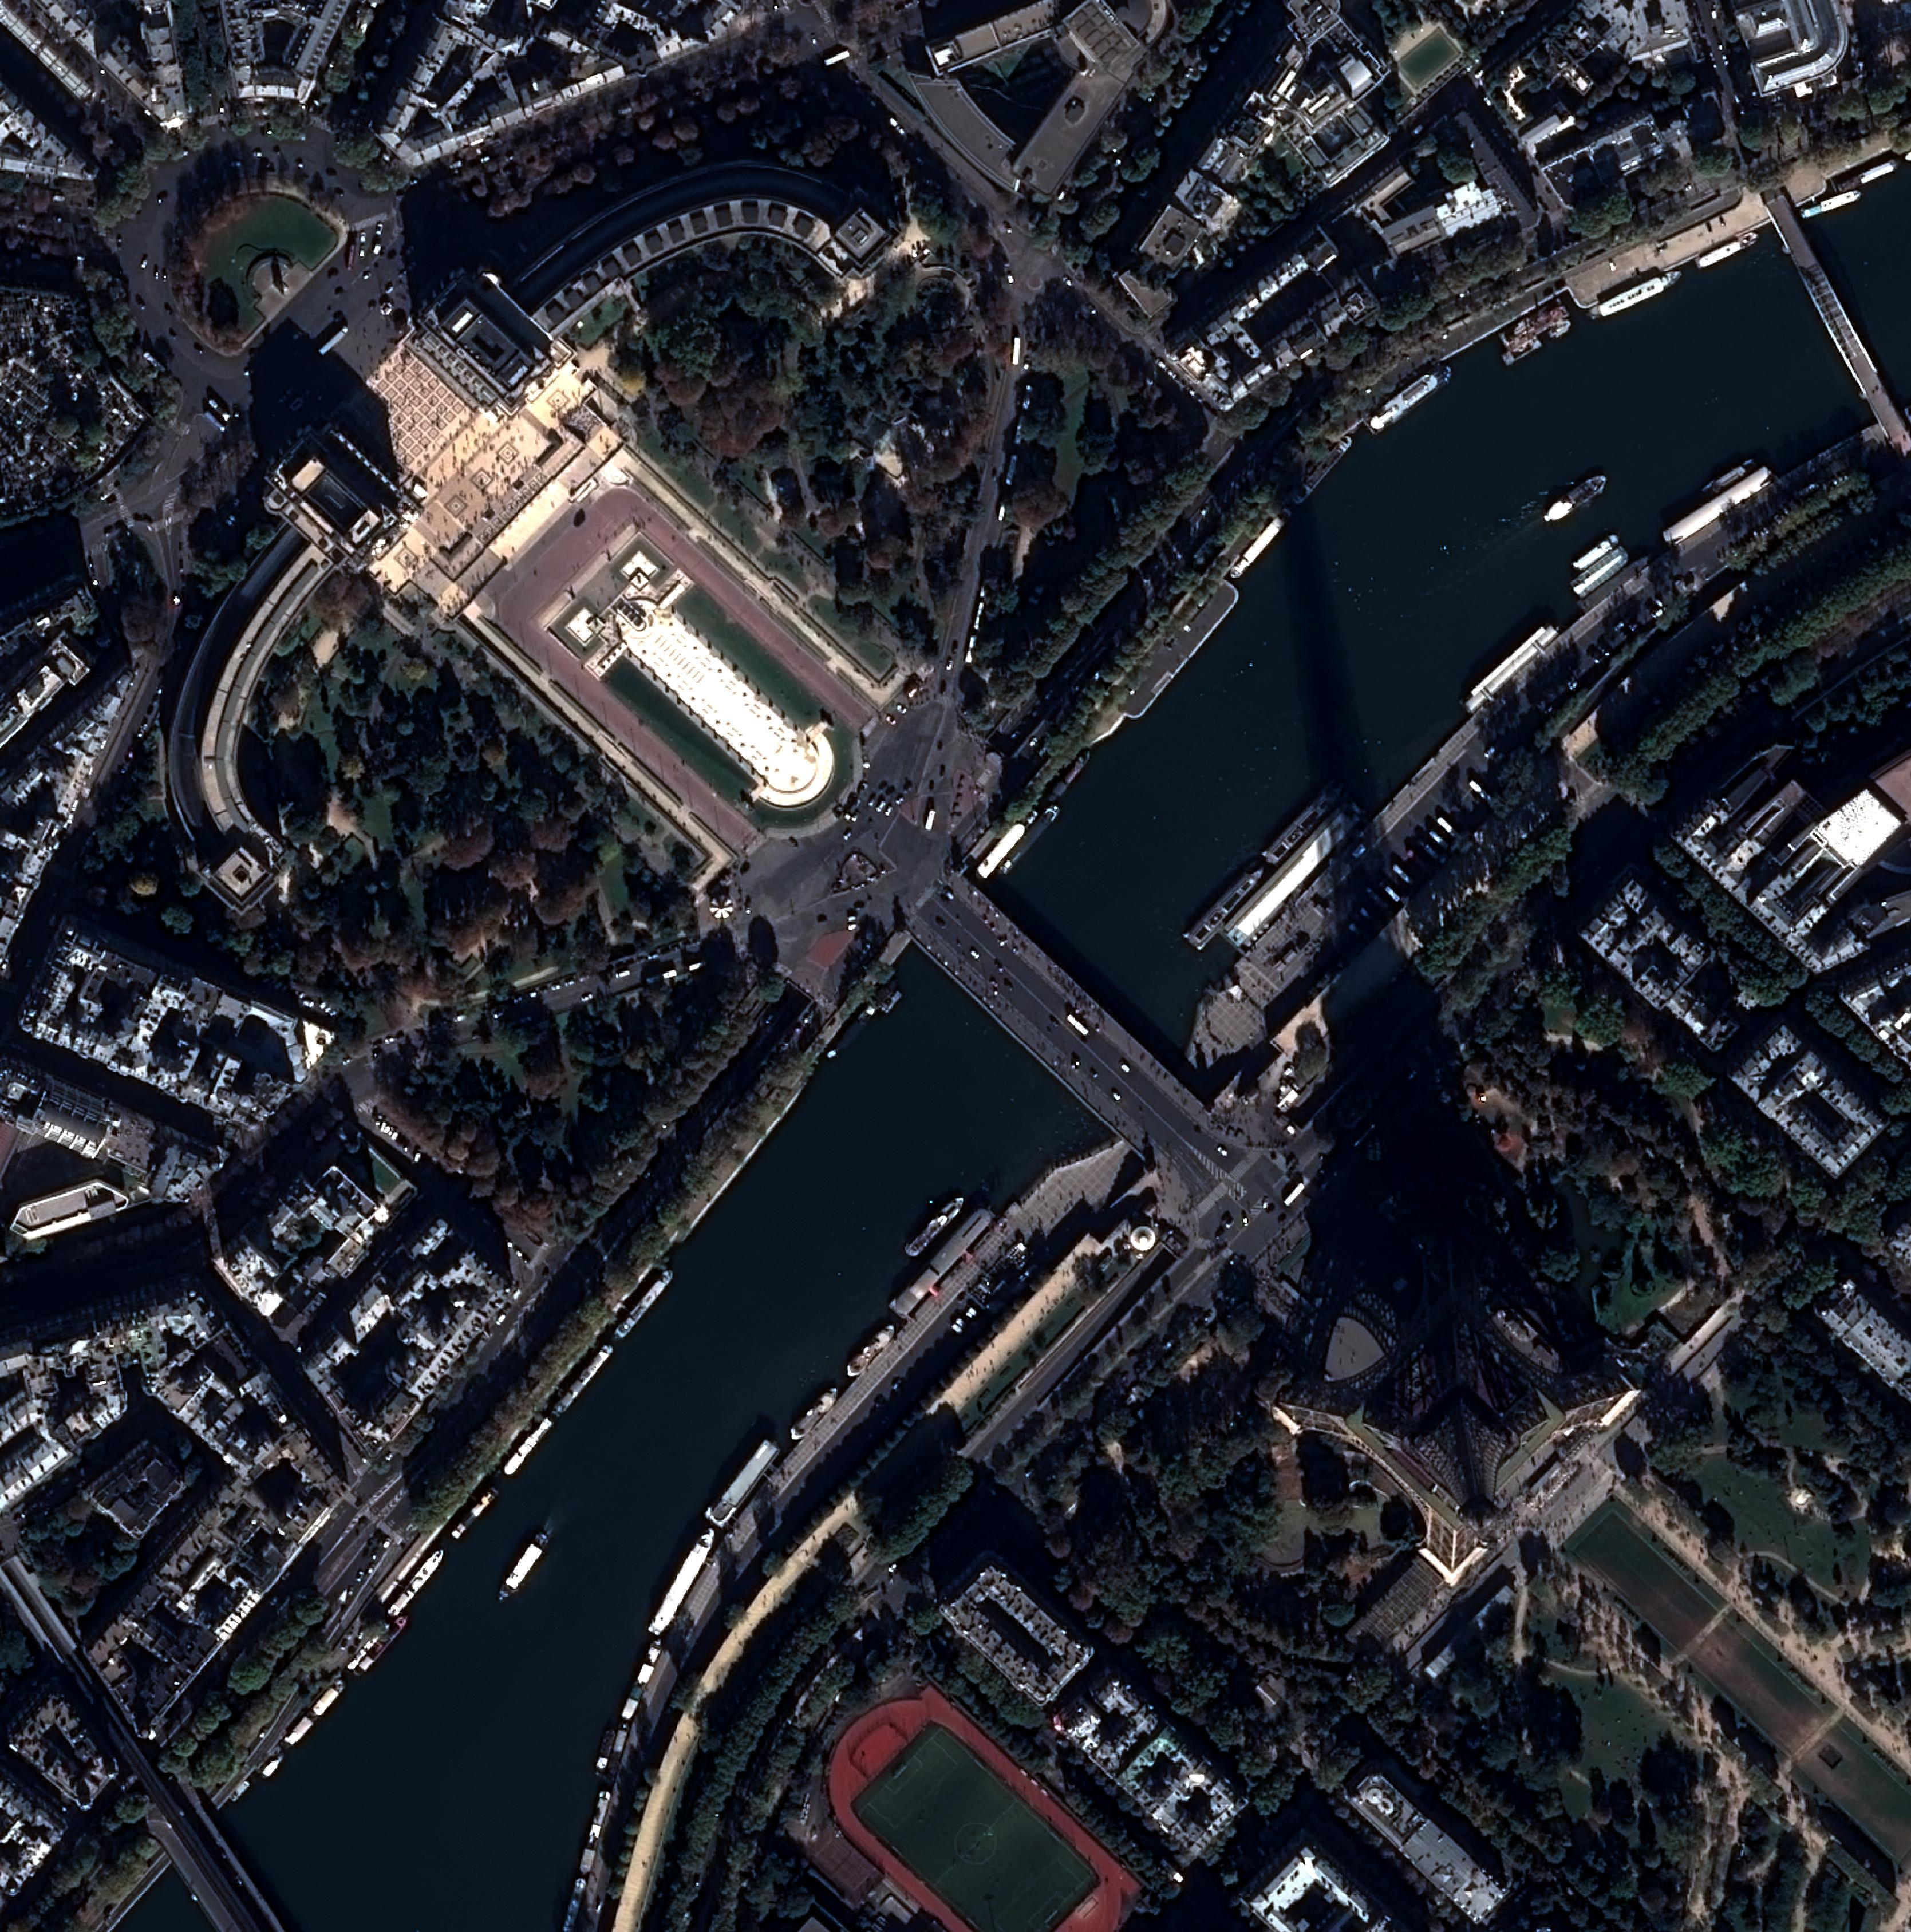
\includegraphics[height=6cm]{Images/Paris_003.jpeg}
        \caption{14/10/2017 11:03:003}
        \label{fig:Pleiade_over_Paris_a}
    \end{subfigure}\hfill
    \begin{subfigure}{0.5\linewidth}
        \centering
        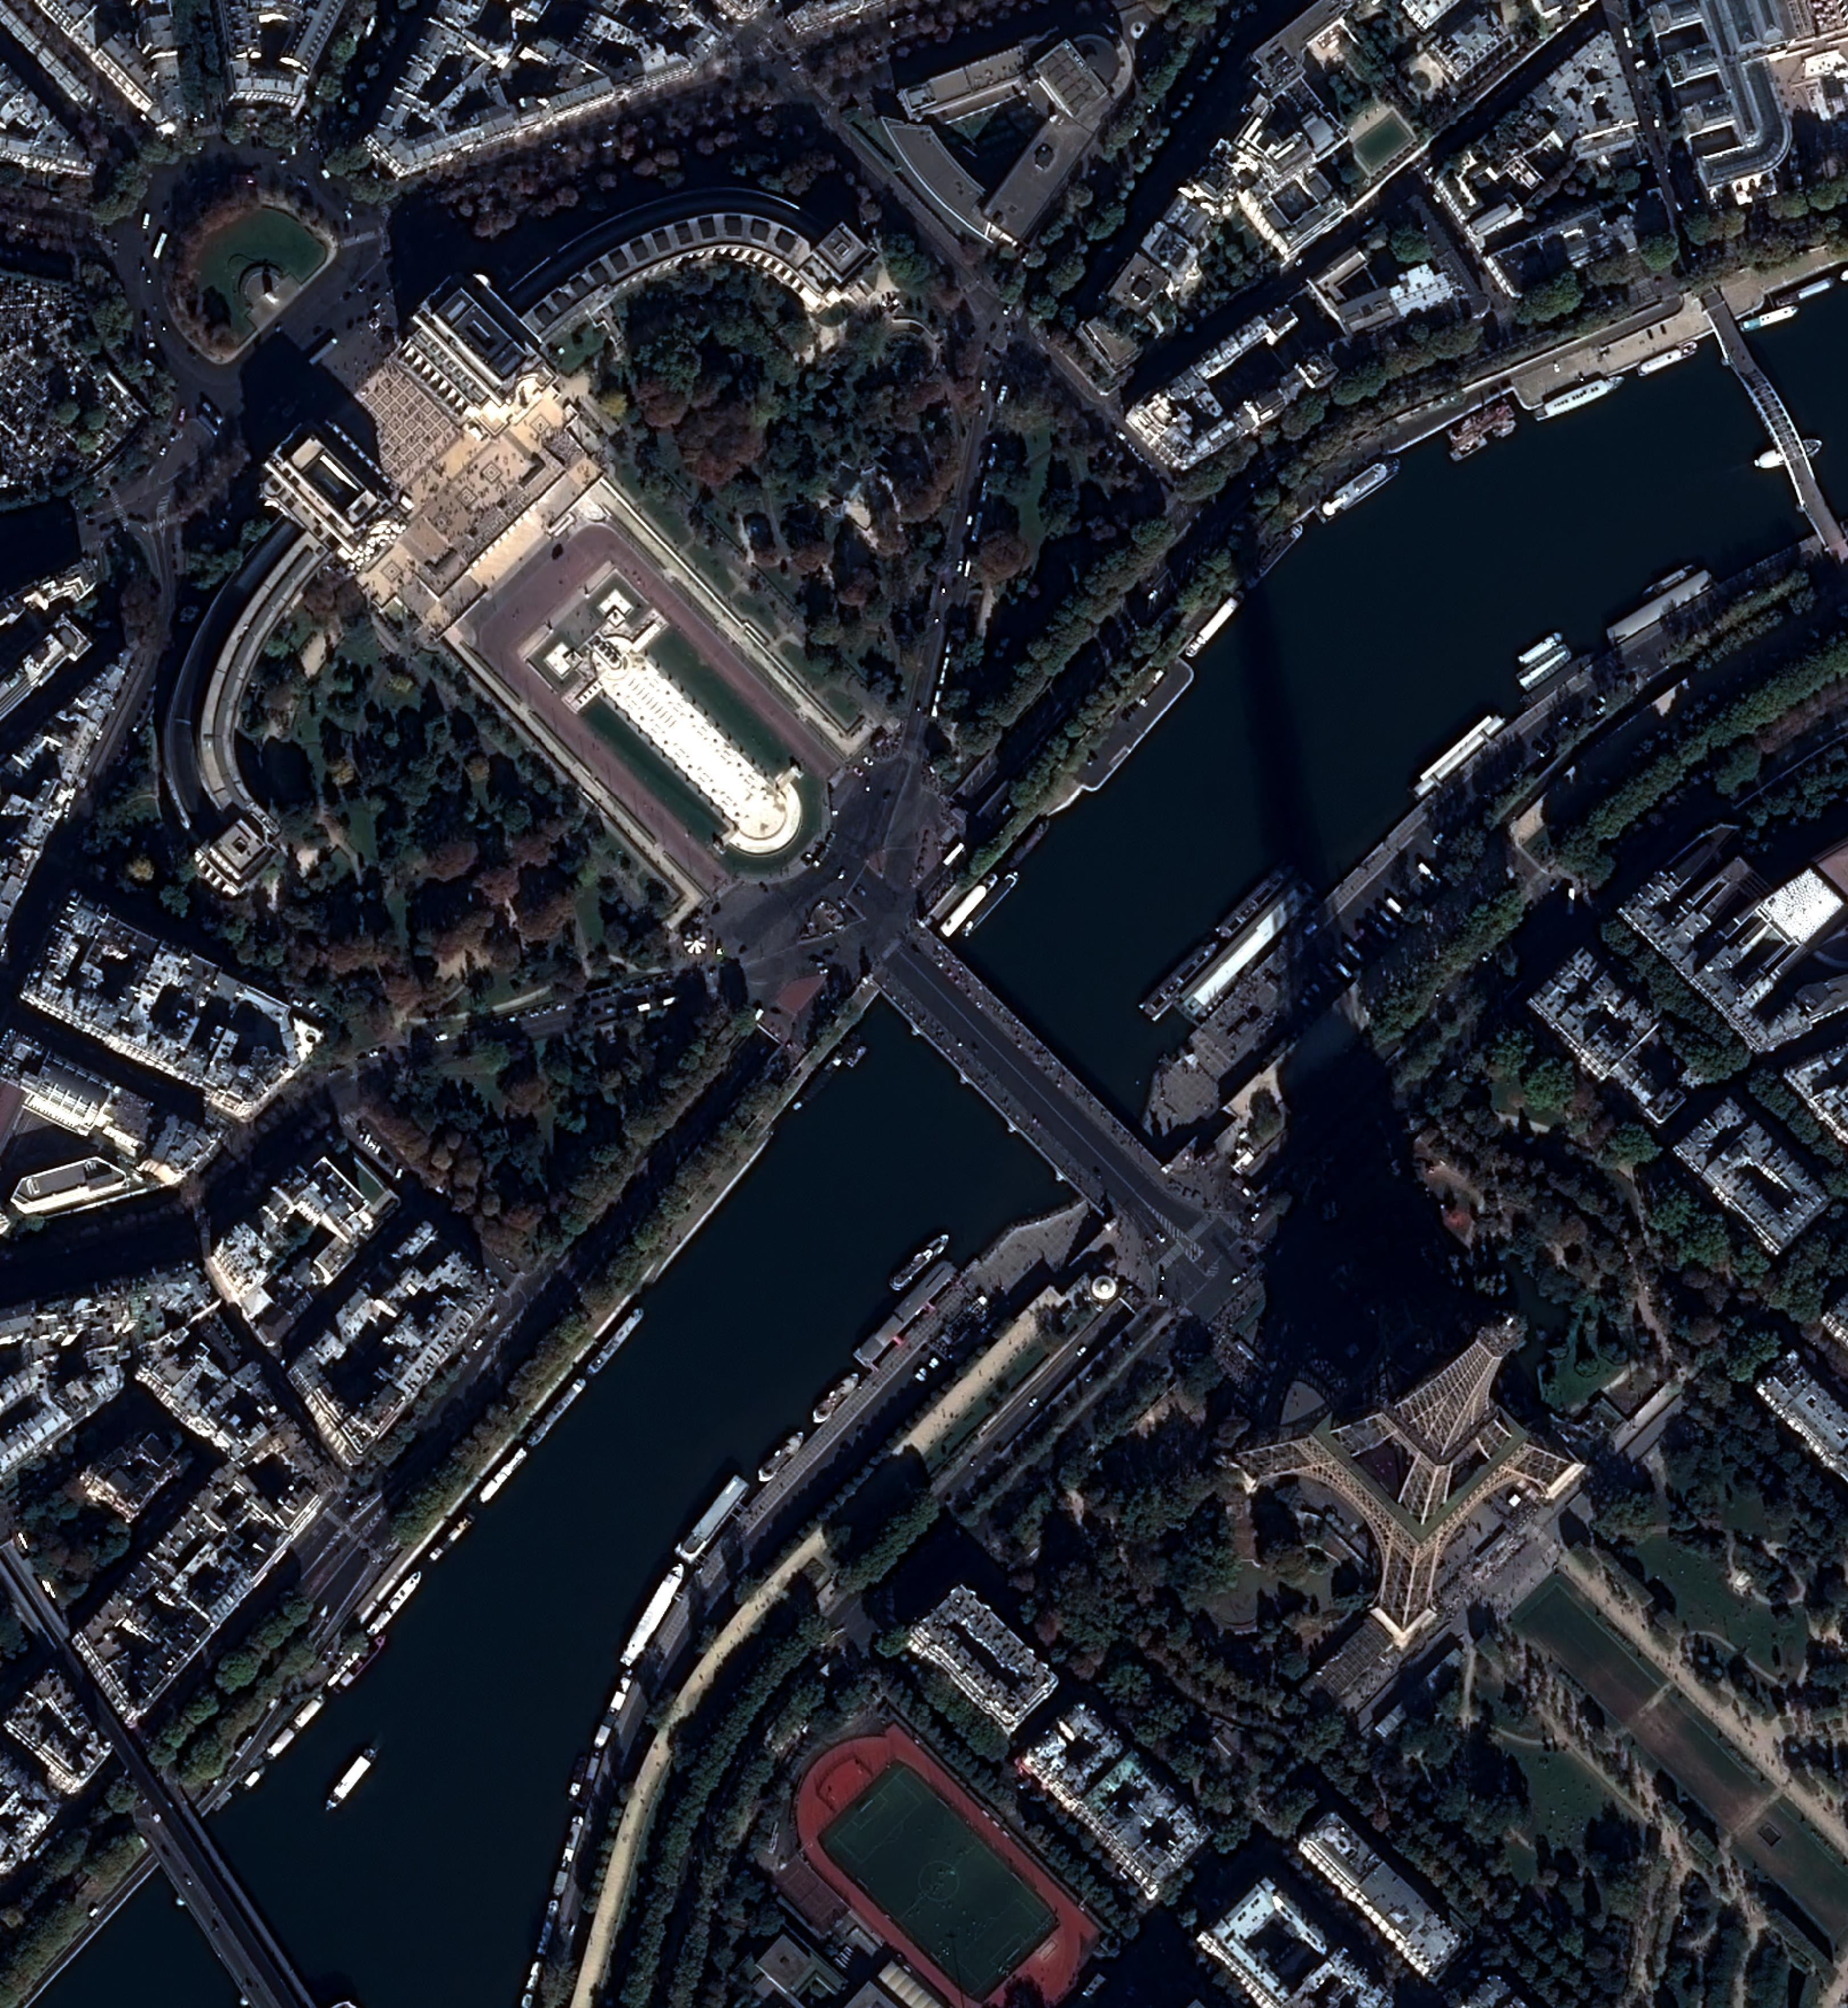
\includegraphics[height=6cm]{Images/Paris_403.jpeg}
        \caption{14/10/2017 11:03:403}
        \label{fig:Pleiade_over_Paris_b}
    \end{subfigure}
    \caption{Pansharpened Pléiades stereo images over Paris at $0.5$m of resolution. Pléiades \copyright CNES 2017, Distribution AIRBUS DS}
    \label{fig:Pleiade_over_Paris}
\end{figure}

In order to produce a worldwide \acrshort{dsm} with $1$m resolution by 2025, the \acrfull{cnes} is launching the \acrfull{co3d} mission \cite{melet_co3d_2020}. Composed of two pairs of low-cost satellites equipped with \acrshort{vhr} optical sensors, the mission will produce image in the \acrshort{rgb} and \acrshort{ir} spectrum at $0.5$m of resolution \cite{lebegue_co3d_2020}. The pairing of satellites allows for \textit{almost} simultaneous stereo image acquisition, cutting short the transient object problem (\ie objects moving/disappearing between stereo images). Different acquisition schemes can also be used, such as the video mode, or even the `diamond' geometry acquisition, which acquires a quadri-stereo over a couple of days. Depending on the relief of the terrain observed, the \acrshort{b/h} ratio will be between $0.2$ and $0.3$. In parallel with image quality specifications, the CO3D products need to abide to a height accuracy of $1$m on low slopes. Another requirement, which is particularly relevant in the context of this thesis, is the production of a performance map supporting the output \acrshort{dsm}. Investigating sources and propagation of the uncertainty inside a 3D stereo pipeline can be beneficial for this performance map requirement. 

\comroman{Parler de Maxar avec les Worldview ?}

\comroman{Schema de la mission CO3D. Type of sensor, push-broom vs raster for CO3D}

One a side note, when an image is acquired both in panchromatic and RGB mode, it is possible to leverage the high resolution of the panchromatic image to improve that of the color image. This fusion technique is called \textit{pansharpening} \cite{loncan_hyperspectral_2015}. We use this technique for clarity in figures and other illustrations of this thesis. It is important to remember that the processed images are the panchromatic images, and not the pansharpened ones which are only used for the final visualization.

\section{Sensors and georegistration}
Different types of sensors can be used to acquire satellite images. Below is detailed a (non-exhaustive) list of sensors of interest \cite{cnes_imagerie_2008}

\textbf{CCD matrix sensor}. CDD are classical sensors used, for instance, in current digital cameras. They possess multiple advantages, such as good geometrical quality as all pixels are acquired simultaneously, or the possibility to perform many acquisitions with various angles possible. However, CCD sensors with small pixel sizes are technologically difficult to built. Augmenting the number of pixels complicates the shutter function, and requires more radiometric calibration as one pixel equals one sensor. It is also more complex to acquire long segments of an image. CO3D satellites will use this technology.

\textbf{Push-broom sensor}. Those image sensors are only composed of a single cell row, acquiring simultaneously radiometric information alongside a line perpendicular to the direction of the satellite. As only one line of cells is needed, push-broom sensors are simple systems which can capture images continuously, while guarantying good geometrical quality along the rows of the images. A variation of those sensors are TDI sensors (Time Delay Integration). Those sensors function as a push-broom except that each row has the ability to transfer its photon charges to the next row. This allows to capture signals over a longer period of time,  thus reducing the signal-to-noise ratio. Harder to produce, TDI sensors also require a precise control of the satellite so that observed objects stay within a column of the TDI sensor. They are used in Pléiades satellites for instance.

A crucial part of satellite imagery is the ability to perform georeferencement, or georegistratation, of every pixel, \ie, locate their coordinates in an Earth system of coordinates such as latitude and longitude. Physical models possess high localisation accuracy, but are sensor-specific and are computationally complex. For stereo reconstruction,  generalized sensor models are preferred. Specifically, we will focus on \acrfull{rpc} \cite{grodecki_ikonos_2001} used by the \acrshort{co3d} and Pléiades satellites. \acrshort{rpc} models are provided alongside images. Sometimes called Rational Function Models \cite{tao_comprehensive_2001}, \acrshort{rpc} are functions allowing to transform a pixel's ground location $(X,Y,Z)$ into its image coordinates $(row, col)$. \acrshort{rpc} encode the line of sight of the satellite, \ie the line joining the center of the sensor's cell to the ground and going through the optical center of the sensor. To improve numerical stability and minimize computation errors, the image coordinates and ground coordinates are normalized between $-1$ and $1$, using their scale factors $SF$ and mean values:
\begin{eqnarray*}
    SF_X &=& \max(X_\mathrm{max}-\overline{X},~\overline{X}-X_\mathrm{min})\\
    \Tilde{X}&=&\frac{X-\overline{X}}{SF_X}
\end{eqnarray*}
The same processed is applied to $Y,Z,row$ and $col$. To avoid heavy notation in this section, we will refer to every normalized coordinate using their non-normalized symbol.

Formally, \acrshort{rpc} are defined as rational fractions of polynomials:  
\begin{eqnarray*}
    \mathrm{RPC}:\mathbb{R}^3 &\rightarrow&\mathbb{R}^2\\
    (X,Y,Z) 	&\mapsto& \left(\frac{Num_{R}(X,Y,Z)}{Den_{R}(X,Y,Z)}, \frac{Num_{C}(X,Y,Z)}{Den_{C}(X,Y,Z)}\right)\\
    &\mapsto&(row,col)
\end{eqnarray*}
where $Num_{R},Den_{R},Num_{C}$ and $Den_{C}$ are the numerators and denominators for rows and columns respectively, expressed as polynomials with a maximum order of $3$:
\begin{eqnarray*}
    Num_R(X,Y,Z) &=& \sum_{i=0}^3~\sum_{j=0}^{3-i}~\sum_{k=0}^{3-i-j}a_{ijk}X^iY^jZ^k\\
    &=& a_{000} + a_{100} X + a_{010} Y + a_{001} Z + a_{110} XY + a_{101} XZ \\
    &&+ a_{011} YZ + a_{200} X^2 + a_{020} Y^2 + a_{002} Z^2 + a_{111} XYZ \\
    && + a_{210} X^2Y + a_{201} X^2Z + a_{120} XY^2 + a_{102} XZ^2\\
    && + a_{021} Y^2Z + a_{012} YZ^2 + a_{300} X^3 + a_{030} Y^3 + a_{003} Z^3
\end{eqnarray*}
$Den_{R},Num_{C}$ and $Den_{C}$ respectively possess different coefficients $a_{ijk}$. The order or indexing of $a_{ijk}$ may differ in the literature. For instance, they can be numbered from $0$ to $19$ or $1$ to $20$, and do not refer to the same indeterminate. \acrshort{rpc} are computed using reference ground control points.

In stereophotogrammetry or ortho-rectification, it is useful to use the inverse \acrshort{rpc} model. As \acrshort{rpc} encode lines of sight, the use of an additional elevation model is required. It can be a geoid modelling the Earth's surface), or a \acrshort{dsm} with higher resolution. Knowing the true elevation $Z$ of a pixel, we define the inverse model as:
\begin{eqnarray*}
    \mathrm{RPC}^{-1}:\mathbb{R}^3 &\rightarrow&\mathbb{R}^3\\
    (row, col, Z) 	&\mapsto& (X,Y,Z)
\end{eqnarray*}

\comroman{Schéma des RPC (voir Grodecki)}

\section{Principle of stereophotogrammetry}
This section dives more into details onto the inner workings of stereophotogrammetry. Photogrammetry is the science of deducing information from photographic images. A sub domain of photogrammetry is stereophotogrammetry, which specifically consists in deducing 3D information from multiple photographic images. Although multiple stereophotogrammetry setups can be achieved, for instance using structured light \cite{scharstein_high-accuracy_2003} or different wavelength \cite{geng_rainbow_1996}, we focus here on the pipelines designed for processing satellite images, which are used and studied in this thesis \cite{franchis_automatic_2014, shean_automated_2016, rupnik_micmac_2017, michel_new_2020}. For more in-depth details on every step of those pipelines, see chapter \ref{sec:classical_stero_pipeline}.

The main idea of stereophotogrammetry for satellite images and other 3D pipelines is to identify the parallax of objects between multiple images, and to deduce the distance between the object and the sensors from this displacement. When expressed in pixels, the displacement is called disparity. To determine this disparity, the images must first be corrected from atmospheric effects (small clouds, aerosols, \etc) to go from top-of-the-atmosphere radiance to the actual light that illuminates the Earth surface \cite{hagolle_maja_2017}, called reflectance. Many stereo setups align their cameras in such a way that objects only move horizontally between images \cite{geiger_are_2012, scharstein_high-resolution_2014, keselman_intel_2017}. This allows to restrict the search space for pixel matches to a single row instead of the whole image. In a way, most people's eyes also present this alignment. When operating satellites, it is more complex to ensure that the sensors disposition will stay consistent, thus requiring some pre-processing step to rectify images and ensuring that the displacement of an object only occurs horizontally. Then matching pixels are determined by computing their disparity. This step is called stereo matching. Usually the depth $z$ of a pixel is computed using the following formula:
\begin{equation}
    z=\frac{Bf}{d}
\end{equation}
where $B$ is the baseline between cameras, $f$ is the focal length of the cameras, and $d$ is the disparity of a pixel. This formula can be found using optical geometry \cite{bolles_epipolar-plane_1987}, and illustrate the fact that pixels closer to the camera present a bigger position shift in between images. In the case of satellite imagery, this relation cannot be used as such. Disparity is used to select the two line of sights joining the object to the cameras, and the object's 3D coordinates are determined by computing lines of sight intersection (or best approximation if they do not strictly intersect). This results in a point cloud, where each point correspond to a match of two pixels. The point cloud can be processed to remove outliers, and is then projected in a regular grid to obtain the desired \acrshort{dsm}.

\comroman{Inclure un schema de TOA radiance?}

Epipolar geometry p128 \cite{cnes_imagerie_2008}

\section{Uncertainty in stereophotogrammetry}
The quality of \acrshort{dsm} obtained using stereophotogrammetry can greatly vary depending on the quality/resolution of the images used, the precision of the georegistration, the performances of the stereo matching algorithm \etc. Reducing the magnitude of errors, or evaluating the uncertainty \textit{a posteriori} has been investigated in multiple work.
Uncertainty on \acrshort{dsm} (global intervals) \cite{hugonnet_uncertainty_2022, deschamps-berger_apport_2021, wang_robust_2015}, \cite{oksanen_digital_2006} \cite{panagiotakis_validation_2018}.Intervals are computed based on a set of reference points (better resolution \acrshort{dsm}, ground truth data).
Fusing \acrshort{dsm} to get better accuracy \cite{qin_uncertainty-guided_2022}
\cite{hu_quantitative_2012,poggi_confidence_2021}
Deep uncertainty for disparity?
In this thesis, we focused on quantifying the uncertainty alongside the creation process of \acrshort{dsm}. We thus differ in this regard from previous work. Our methodology estimates the uncertainty independently for every pixels, 

\section{Classical stereo pipeline}\label{sec:classical_stero_pipeline}
\subsection{Resampling in epipolar geometry}
SIFT computation, sparse matching, rectification grid
\subsection{Stereo matching}
Optical demonstration for disparity to height
Taxonomy. Cost functions. SGM. Deep learning methods
\subsection{Triangulation}
RPC models. Line of sight intersection
Filtering of point clouds
\subsection{Rasterization}
Gaussian rasterization. Holes filling.  
\subsection{From LiDAR to disparity GT}
Explaination on how to obtain GT disparity maps from georeferenced LiDAR, \cite{cournet_ground_2020}. Line of sight and default geoid. 

\pagebreak